\documentclass[tikz,border=2pt]{standalone}
\usepackage{tikz}
\usepackage[european]{circuitikz}
\usetikzlibrary{arrows.meta,positioning,calc}
../cictikz/src/cictikz/data/tex/cictikz_lib.tex
\begin{document}
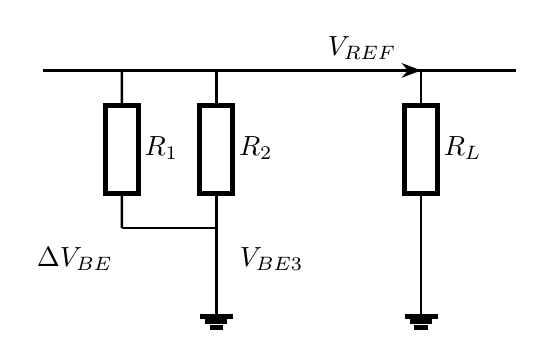
\begin{tikzpicture}[>=Stealth, line width=0.9pt]
  \draw (0,2.6) -- (6,2.6);
  \draw (1.0,2.6) to[resistor,l=$R_1$] (1.0,0.6);
  \draw (2.2,2.6) to[resistor,l=$R_2$] (2.2,0.6);
  \draw (1.0,0.6) -- (2.2,0.6) -- (2.2,-0.1) node[ground] {};
  \node at (0.4,0.2) {$\Delta V_{BE}$};
  \node at (2.9,0.2) {$V_{BE3}$};
  \draw[->] (3.3,2.6) -- (4.8,2.6) node[midway,above] {$V_{REF}$};
  \draw (4.8,2.6) to[resistor,l=$R_L$] (4.8,0.6) -- (4.8,-0.1) node[ground] {};
\end{tikzpicture}
\end{document}
